\documentclass[12pt]{article}
\usepackage{amsmath,amsfonts,fullpage,amsthm,graphicx,verbatim}

\newtheorem*{theorem}{Theorem}
\newtheorem*{fact}{Fact}
\newtheorem*{goal}{Goal}
\newtheorem*{idea}{Idea}
\newtheorem*{defn}{Definition}
\newtheorem*{ex}{Example}

%Style section
%\setlength{\textheight}{10in}
%\setlength{\textwidth}{7in}
%\hoffset=-0.75in
 \pagestyle{plain}
% \setlength{\topmargin}{0in}
% \setlength{\headsep}{0in}
% \setlength{\oddsidemargin}{0in}
% \setlength{\evensidemargin}{0in}

\begin{document}


\pagestyle{empty} %use this to get rid of page numbers

\noindent
{Math 166  \hskip 1.5 truein  Names:\ \hrulefill}

\noindent
%\vskip 0.3truein
%\bigskip
%\noindent
{Trig integration}

\noindent  \hskip 3.5 truein  Section Number:\ \hrulefill
\smallskip

\begin{goal} \rm
Figure out how to evaluate trig integrals 
\end{goal}


\begin{enumerate}
\setcounter{enumi}{-1}
%\item (Trig review) Write down expressions for $\tan$, $\cot$, $\sec$, and $\csc$ in terms of $\sin$ and $\cos$.
%\vspace{1.25in}

%\item Starting with everyone's favorite trig identity, $\sin^2 x + \cos^2 x = 1$, do some algebraic manipulation to write down two different identities involving $\tan^2$, $\cot^2$, $\sec^2$, and/or $\csc^2$. (Hint: we found one of these identities in class yesterday)
%\vspace{1.25in}

\item If we were using $u$-substitution and we set $u=$ one of the six trig functions, then $du=$? 

\noindent
\begin{align*}
u &= \sin (x) \hspace{1.025in} du = \hspace{1.25in} u = \sec (x) \hspace{1in} du = \\
u &= \cos (x)\hspace{1in} du = \hspace{1.25in} u = \csc (x) \hspace{1in} du = \\
u &= \tan (x)\hspace{.975in} du = \hspace{1.25in}
u = \cot(x) \hspace{1in} du = 
\end{align*}

\item Evaluate the following integrals using one of the substitutions from Exercise $0$. You may need to use some trig identities and/or simplify first.
\begin{enumerate}
\item $\displaystyle\int  \tan (x) \sec^3 (x) \ dx$

\vspace{2in}

\item $\displaystyle\int \tan^2 (x) \sec^4 (x) \ dx$

\vspace{2in}

%\item $\displaystyle\int \tan^4 x \sec^3 x \ dx$

%\vspace{1.25in}

%\end{enumerate}

%\noindent (What conditions do we need on $m$ and $n$ to be able to evaluate $\displaystyle\int \tan^m  \sec^n x \ dx$ using one of the substitutions from Exercise $0$?)

\pagebreak
%\vspace{.5in}

\item $\displaystyle\int {\sin (3x) \tan^2 (3x)}\ dx$


\vspace{2in}

\item $\displaystyle\int \cos^{5/2} (4-x) \sin^5 (4-x) \ dx$

\vspace{2in}

\item $\displaystyle\int \cot^3 (x) \csc (x) \ dx$

\vspace{2in}

\item $\displaystyle\int \frac{\cos^2 (x)}{\sin^4 (x)}\ dx$

\vspace{2in}

\end{enumerate} 

\newpage
%\begin{comment}
%\vspace{1.25in}

%\end{comment}

\item Evaluate the integral by the following steps.
\[\displaystyle\int  \frac{1}{x^4\sqrt{x^2-4}} \ dx\]
\begin{enumerate}
\item First, substitute $x=2\sec(\theta)$ (this is a \emph{trig substitution} which will discuss next lecture). Convert the integral completely into the variable $\theta$. (Hint: If $x=2\sec(\theta)$ then what does $dx$ equal?) 

\vspace{1.25in}
\item Use the trig identity $\tan^2(\theta)+1=\sec^2(\theta)$ to simplify the denominator by making the part under the square root into a perfect square. (This kind of simplification is the goal of trig substitution.) Then evaluate the integral.

\vfill
\vfill
\vfill

\item Convert back to the variable $x$ by using our trig substitution $\sec(\theta)=\frac{x}{2}$ and the definition of the trig functions in terms of a right triangle.

\medskip
\begin{center}
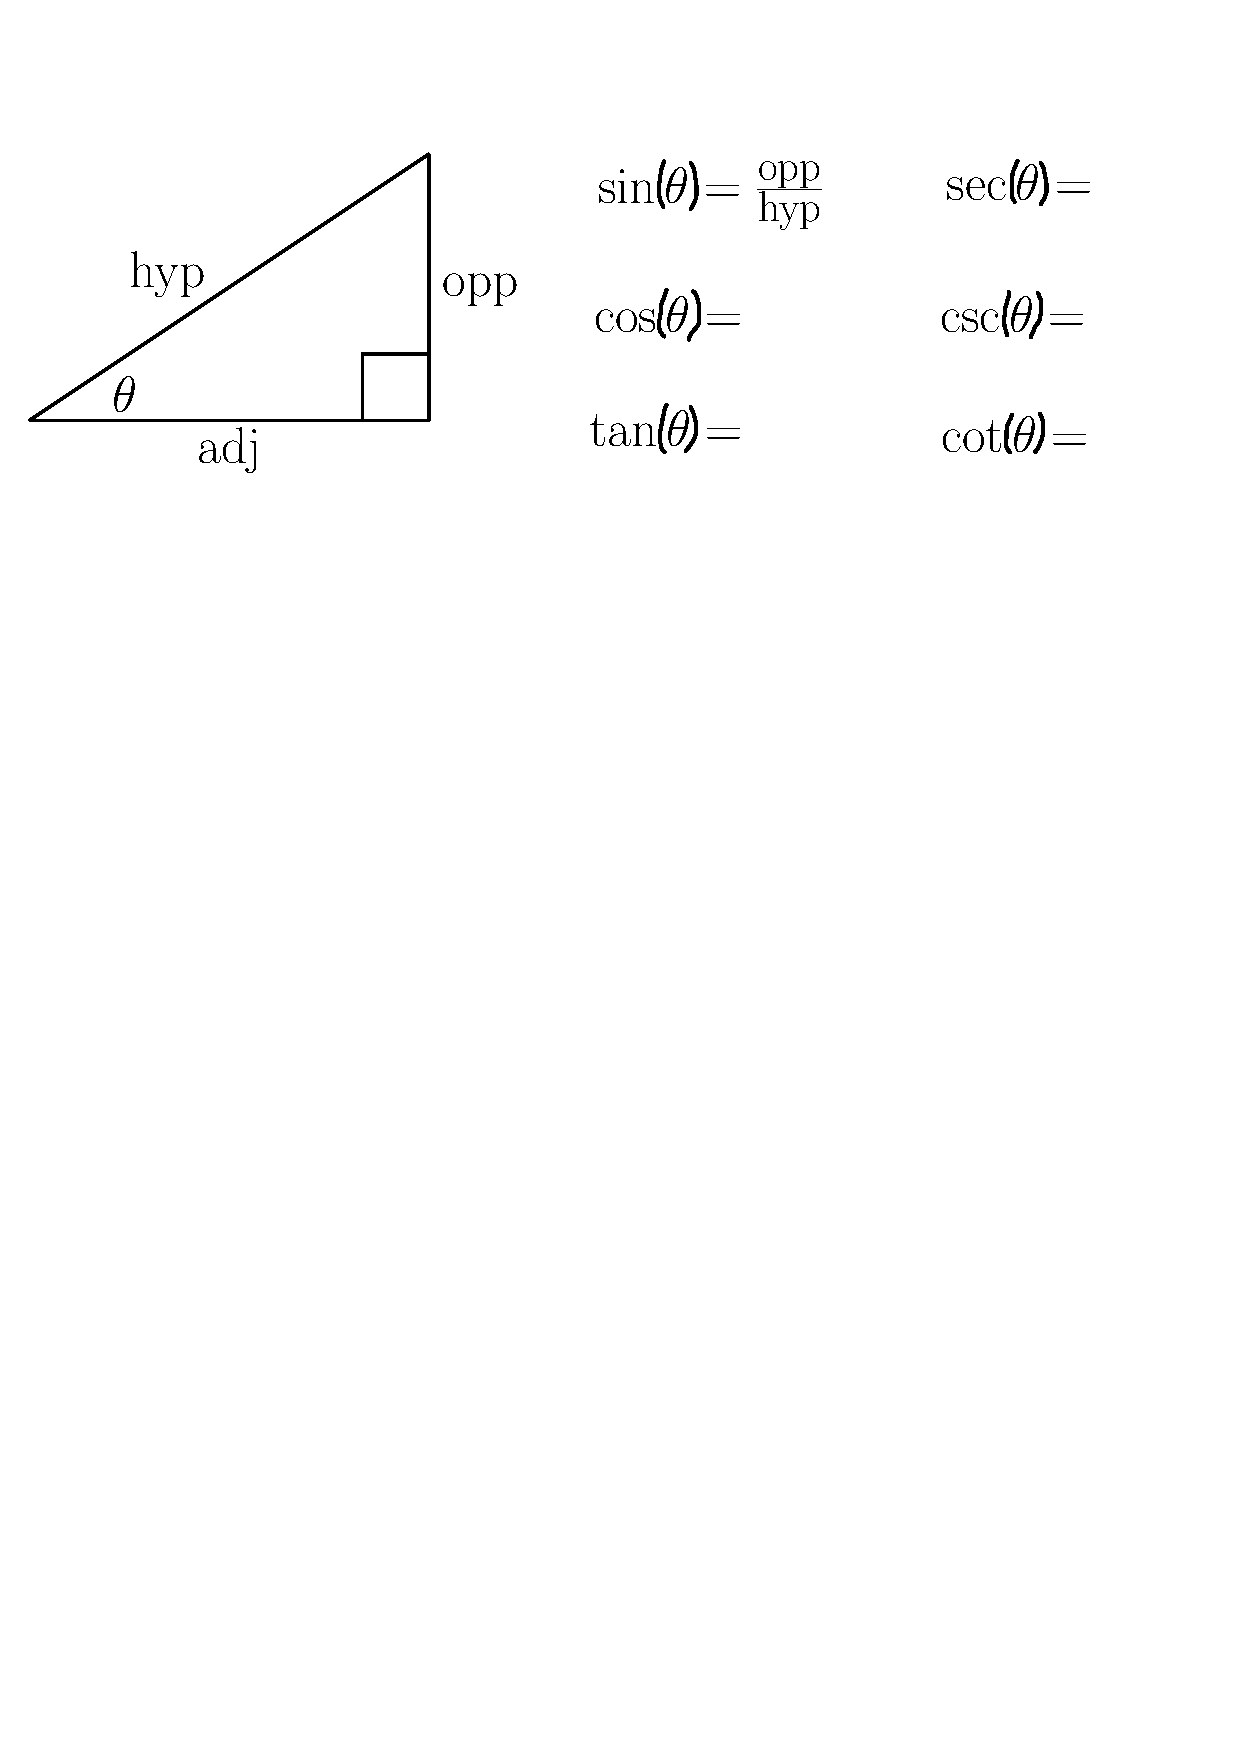
\includegraphics[scale=.65]{right_triangle.pdf} 
\end{center}

%\item Write your answer in terms of the variable $x$.

\end{enumerate}
\end{enumerate} 

\end{document}
